\section{The goals of thesis}
The tool was created mainly for didactic purposes -- its purpose is to facilitate visualization and thus understand for a novice programmer the operation of algorithms created in C-based languages by directly showing the flowchart diagram related to the written code. Additionally, it is a handy tool that allows to create flowcharts easily and quickly, requiring only the basics of programming for various purposes. The tool should also enable users to easily share diagrams with other users in a form that can be easily edited further.
	
\section{Examples of existing solutions for drawing flowcharts}

	\subsection{Raster graphic editor} 
	The use of any graphics editor -- this is the least efficient solution - drawing diagrams in this way is time-consuming and difficult to edit. It also requires a good knowledge of the editor from the user. The only advantage compared to other solutions is that the final result is not limited to predefined forms -- it gives the greatest freedom.
		
	\subsection{Tools for manual creation of diagrams} 			
	A tool specially designed for drawing various types of diagrams including flowcharts by manually placing individual blocks, describing and connecting them, e.g. \href{https://www.lucidchart.com/pages/examples/flowchart_software}{lucidchart} -- much more efficient than when using a raster graphics editor thanks to the predefined elements that the user can place and edit to a fairly large extent.
	
	\subsection{Code to flowchart converter} 	
	\begin{itemize}
	\item
	A tool with its own syntax, created especially for drawing flowchart diagrams. The syntax itself is usually quite simple, but the code required to create the flowchart in no way relates to the algorithm it represents, and in more complex cases it is unreadable, which makes the user's work much more difficult and inefficient. One of the many examples of such a tool is \href{https://mermaid-js.github.io/mermaid/#/}{Mermaid} -- used further in this project as an intermediary language between the input of C-based code and the final output in the form of a flowchart in an HTML page.
	
	\item
	Converter of pseudoprogramming code directly into a flowchart diagram (a variant of which is this project). A commercial version of such a converter is available on the market under the name \href{https://code2flow.com}{code2flow}. The advantage of these solutions is the many times the higher efficiency of drawing the diagram and its direct reference to the written code, which gives a better guarantee of the correctness of the solution and the easiest edition of all available methods described before. The only disadvantage of this method is its low flexibility -- the user has little influence on the final appearance of the diagram, it is largely predefined by the creators of this type of tool.
	\end{itemize}
	
\begin{figure}[h]
    \centering
\begin{minipage}[b]{.33\textwidth}
    \centering
   %\begin{flalign} 
   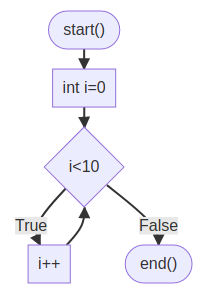
\includegraphics[width=.9\linewidth]{decyzja-while.png}
   %\end{flalign}   
\end{minipage}%
\hfill\vline\hfill
\hspace{0.02\linewidth}
\begin{minipage}[b]{0.3\textwidth}
    \centering 
%\begin{flalign}
\strut\vspace*{-\baselineskip}\newline\
C:
\begin{minted}{cpp}
  
start();
int_ i = 0;
while(i < 10){
  i++;
}
end();
  \end{minted}
%\end{flalign}
\end{minipage}%
\hfill\vline\hfill
\hspace{0.02\linewidth}
\begin{minipage}[b]{0.3\textwidth}
    \centering
    %\begin{flalign}
    \strut\vspace*{-\baselineskip}\newline\
    Mermaid:
  	\begin{minted}{python}
graph TD;
N1(["start()" ]);
N2["int i=0" ];
N5{"i<10" };
N6["i++" ];
N7(["end()" ]);
N1-->N2;
N2-->N5;
N5-->|True|N6;
N5-->|False|N7;
N6-->N5;
  	\end{minted}
   %\end{flalign}

    \end{minipage}
    \label{fig:prob3}
    \caption{Comparison of the syntax of both types of converters that generate the same flowchart diagram.}
\end{figure}
	

	
\section{Form of the project}
The thesis is a project and consists in creating a tool with which it will be possible to easily draw (generate) flowcharts based on syntax elements taken from the C language, such as:

\begin{itemize}
	\item {
		function call or assignement operation -- as process block
	}
	\item conditional statement of type $if / else$ -- a decision block with two branches representing the execution of subsequent instructions depending on the condition specified inside the decision block,
	\item  conditional statement executing the $while$ loop -- as a decision block, along with a loop pointing to this block after the completion of the instructions listed inside the scope of the statement.
\end{itemize}

The generator (similarly to the C language compiler) supports the nesting of the above statements (i.e., you can extend the decision tree by placing one conditional statement inside another). The application is able to interpret only the above-mentioned instructions, which are sufficient to create most of the algorithms in practice. The deviations and shortcomings compared to the C language are the lack of such statements as: for, do-while and goto. From the point of view of the algorithm itself, each for and do-while loops can be replaced with the most basic while loop - in the case of for: declaration of additional variables before the loop and execution of an additional statement at the end of each iteration of the loop. As in the case of do-while: replacement of the main condition of the loop with the inner conditions to call continue or break statements. The goto statement is omitted because it is fully replaceable with loops, it is also considered a bad programming practice to use it. In addition, due to the fact that the application interface is an HTML form that sends requests to the server through the Rest API, after making the application available, e.g., on a cloud service, it will be possible to easily share the created diagram along with the code on the basis of which it was created using the URL link. An additional functionality is also support for Unicode characters, which allows you to write code using, among others, Polish characters and text wrapping in blocks, preventing excessive block growth with larger amounts of text.
  
\section{Used tools and technologies with description }
All the listed technologies and tools used are open-source and do not require any additional obligations for their use:

\begin{itemize}
	\item HTML5, CSS, Thymeleaf -- the user interface of the application will be a simple HTML form on a website obtained using the HTML template method, communicating with the server via the HTTP protocol and the Rest API.	
	
	\item Mermaid -- a tool developed in JavaScript that allows to draw diagrams on an HTML page using a special syntax, unique for this tool.
	
	\item Java 11 SE, Spring Boot framework -- the back-end part of the application in which, among others include: support for Rest API queries, implementation of classes and algorithms contained in them that interpret the C-based language and convert it into the language required by the diagram drawing tool used (Mermaid in this case)
	
	\item Used programming tools: IntelliJ IDEA Community Edition, Visual Studio Code, Git as version control system .
		
		
\end{itemize}
	